\subsection{Encoding}
\label{sec:math_encoding}

Some elliptic curve based cryptosystems (such as the adapted ElGamal in Section \ref{sec:math_encryption}) are constructed to encrypt points on a curve. To make
this useful an original string message must be encoded as a point. The encoding must be reversible and have a one-to-one relationship between encoded and raw
messages.

It should be noted that Bouncy Castle does not, at the time of writing, contain any implementations of encoding algorithms.

It is trivial to map a message string to the correct numberspace as both strings and numbers have binary representations. The number is then
simply found by converting a string to its binary representation and interpreting this as an integer. Using the ASCII character set the string
\verb+"A"+ is mapped to the number \verb+65+.

\begin{verbatim}
    string_to_binary "A" -> 1000001
    binary_to_integer 1000001 ->  65
    
    string_to_integer m = binary_to_integer (string_to_binary m)
    string_to_integer "A" -> 65
\end{verbatim}

Indeed, any string \(m\) may be transformed to an integer \(M\) using this method.

Koblitz is attributed with an algorithm that maps a message \(m\), represented as an integer in \(\mathbb{Z}_p\), to a point on the curve of the
simple Weierstrass form \(y^2 = x^3 + ax + b \text{ mod } p\).\footnote{While other encoding algorithms, which offer better performance and probability
for successful encoding, do exist,\cite{MappingAMessage}\cite{InjectiveEncodings} the encoding algorithm described here offers so high probability
and performance (see Section \ref{sec:performance_components}) that implementing any more algorithms was not a priority.}\cite{MappingAMessage}

An integer K is selected such that \((M + 1)K < p\), and this is used to compute
a candidate x-coordinate for the point, \(x_j = MK + j \text{ mod } p\). To verify the validity of the candidate, a check is performed: \(x_j\)
is a valid x-coordinate for a point on the curve if \(z_j = x_j^3 + ax_j + b\) has a square root. If the candidate is valid, the message \(m\)
can be mapped to a point \(M\) on the curve:

\begin{equation}
	M = (x_j, y_j) \text{, where } y_j = \sqrt{z_j} \text{ mod } p
\end{equation}

If no square root exists for \(z_j\) for all \(j \in \{0,1,...,K-1\}\), then it is not possible to map the message to a point. In other
words, the method is probablistic and it is possible that a message cannot be encoded.

The original message can be found from the point by performing a simple calculation:

\begin{equation}
	m = {\lfloor {x \over K} \rfloor}
\end{equation}

The flooring of \(x \over K\) ensures that any \(j\) added to \(MK\) has no effect.\cite{MappingAMessage}

As the numberspace the messages must be mapped to is limited by the size of the prime field \(\mathbb{F}_p\) over which the curve is defined, so is the
length of the message. The numeric value \(M\) of a string can be no greater than \(p\).

\paragraph{Picking the value K}

The selection of value \(K\) has implications on both the probability that a message can be mapped, and the performance of the encoding algorithm.
The probability of successful encoding is described as \(P_{success} \geq 1 - {1 \over {2^K}}\): the larger the value of \(K\), the greater the probability,
as shown in Figure \ref{fig:probability}. With \(K\) greater than 6, no discernible change in probability occurs.\cite{MappingAMessage}

\begin{figure}[htb]
	\centering
	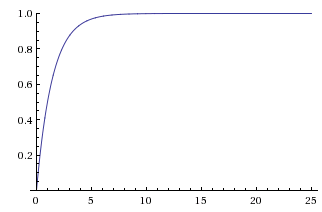
\includegraphics[width=0.6\textwidth]{maths/encoding-probability}
	\caption{Minimum probability of successful encoding, depending on size of K: \(P_{success} \geq 1 - {1 \over {2^K}}\).}
	\label{fig:probability}
\end{figure}

The performance of the mapping depends on three calculations: (1) the multiplication \(MK\); (2) the calculation of \(z_j\), specifically
performing the calculations \(x_j^3\) and \(ax_j\); and (3) the computation of a potential root \(\sqrt{z_j}\). While the first calculation (1)
is performed only once, the last two (2,3) are repeated until a root is found, or all possible values have been tried.

Multiplication is a heavy operation, and picking a smaller value of \(K\) limits both the load of each multiplications (as they are performed with
smaller numbers), and the number of multiplications (as the range of \(j\)s used is limited by \(K - 1\)). So while it is easy to find the greatest
possible value \(K_{greatest} = {\lfloor { p \over {M + 1} }\rfloor}\) yielding the highest probability of success, this is not necessarily desirable.

For example, the curve \verb+secp256k1+ has a prime that can be approximated as \(p_{secp256k1} \simeq 1.16*10^{77}\).\cite{safecurves} An M can be
found from a message of a reasonably short length: \(M = \mathtt{string\_to\_integer(``Hello, World.")} \simeq 3.68*10^{30}\). This would lead to
\(K_{greatest} \simeq {\lfloor { {1.16*10^{77}} \over {3.68*10^{30} + 1}} \rfloor} = 3.15*10^{46}\), which would lead to a huge amount of multiplications.

Picking \(K = 7\) gives a probability of success \(P_{success} \geq 0.993\), leaving less than a \(0.7\%\) failure rate.